\documentclass[tikz,border=5pt]{standalone}
\usetikzlibrary{arrows.meta,positioning,shapes.geometric}
\begin{document}
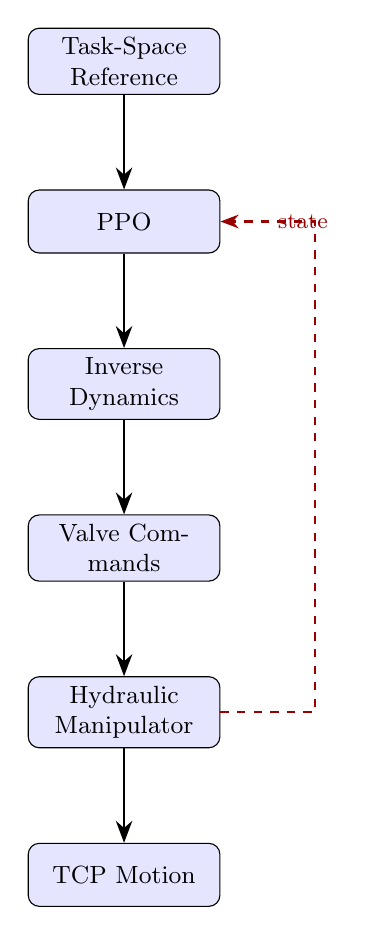
\begin{tikzpicture}[
    node distance=1.2cm,
    block/.style={rectangle,draw,fill=blue!10,text width=2.2cm,text centered,rounded corners,minimum height=0.8cm,font=\small},
    arrow/.style={-{Stealth[scale=1.2]},thick},
    feedback/.style={-{Stealth[scale=1.0]},thick,dashed,red!60!black},
]

\node[block] (ref) {Task-Space Reference};
\node[block,below=of ref] (ppo) {PPO};
\node[block,below=of ppo] (id) {Inverse Dynamics};
\node[block,below=of id] (valve) {Valve Commands};
\node[block,below=of valve] (plant) {Hydraulic Manipulator};
\node[block,below=of plant] (tcp) {TCP Motion};

\draw[arrow] (ref) -- (ppo);
\draw[arrow] (ppo) -- (id);
\draw[arrow] (id) -- (valve);
\draw[arrow] (valve) -- (plant);
\draw[arrow] (plant) -- (tcp);

\draw[feedback] (plant.east) -- ++(1.2,0) |- (ppo.east)
    node[pos=0.75,right,font=\footnotesize] {state};

\end{tikzpicture}
\end{document}
